\documentclass[a4paper,11pt,oneside,openany]{jsarticle}
\usepackage[dvipdfmx]{graphicx}
\usepackage{amsmath,amssymb}
\usepackage{bm}
\usepackage{graphicx}
\usepackage{ascmac}
%
% \setlength{\textwidth}{\fullwidth}
% \setlength{\textheight}{40\baselineskip}
% \addtolength{\textheight}{\topskip}
%\setlength{\voffset}{-0.55in}
\thispagestyle{empty}
%
\begin{document}
\begin{center}

  \vspace*{40mm}
  \huge 計算機科学実験及演習3 \par
  機能設計仕様書\\
  \vspace{90mm}
  \Large 提出期限:2019/5/9\\
   提出日: \today \\
  \vspace{15mm}
  \Large グループ番号: 9    \\
   1029293806\hspace{5mm}大山 偉永\par


  \vspace{10mm}
\end{center}
\clearpage
\addtocounter{page}{-1}

\newpage

\section{コンポーネント分割}
\begin{figure}[h]
  \centering
  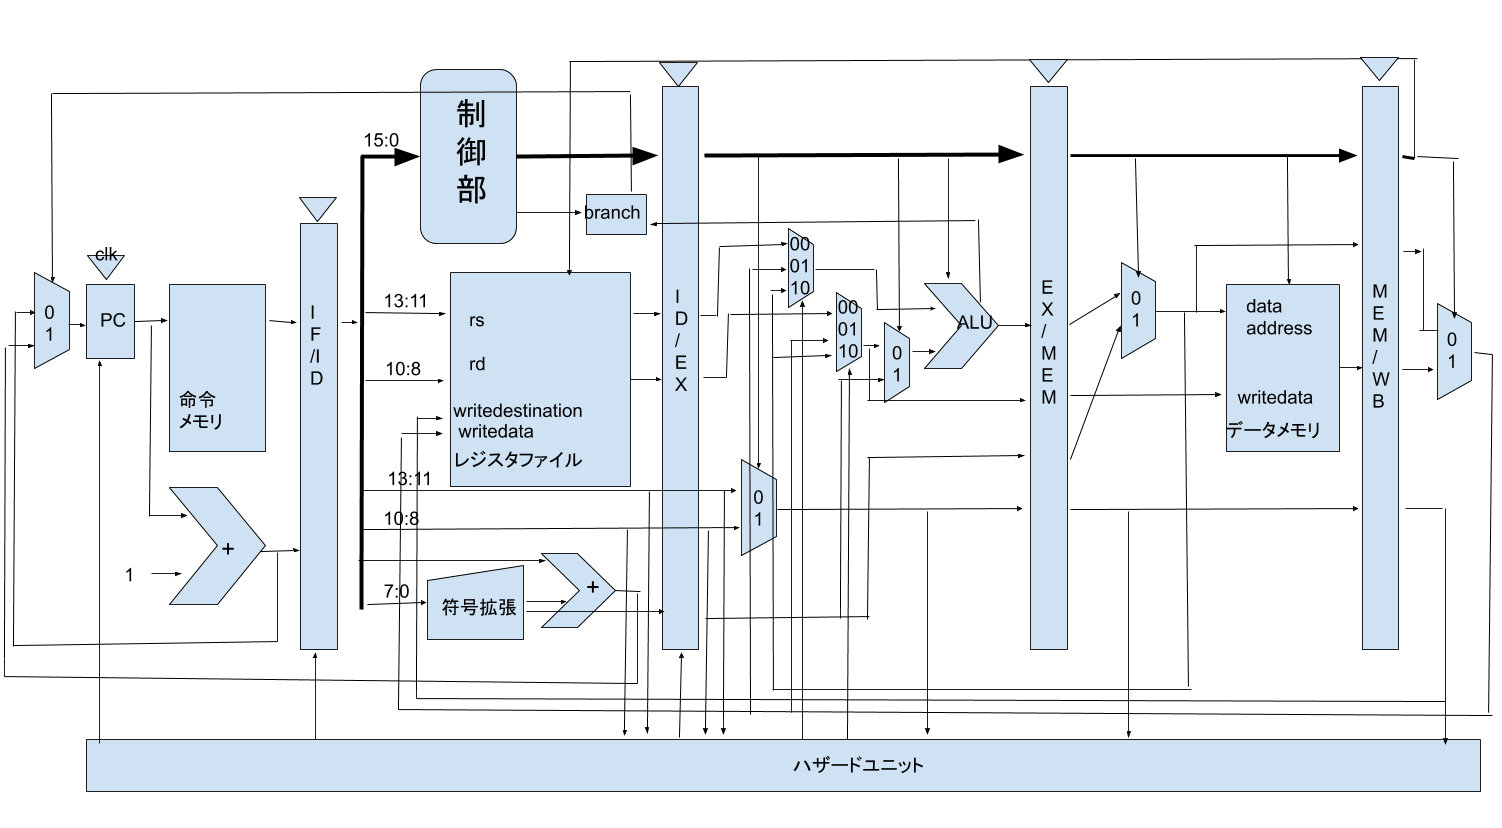
\includegraphics[width=12cm]{block.png}
  \caption{全体のブロック図}
  \label{block}
\end{figure}
\begin{figure}[h]
  \centering
  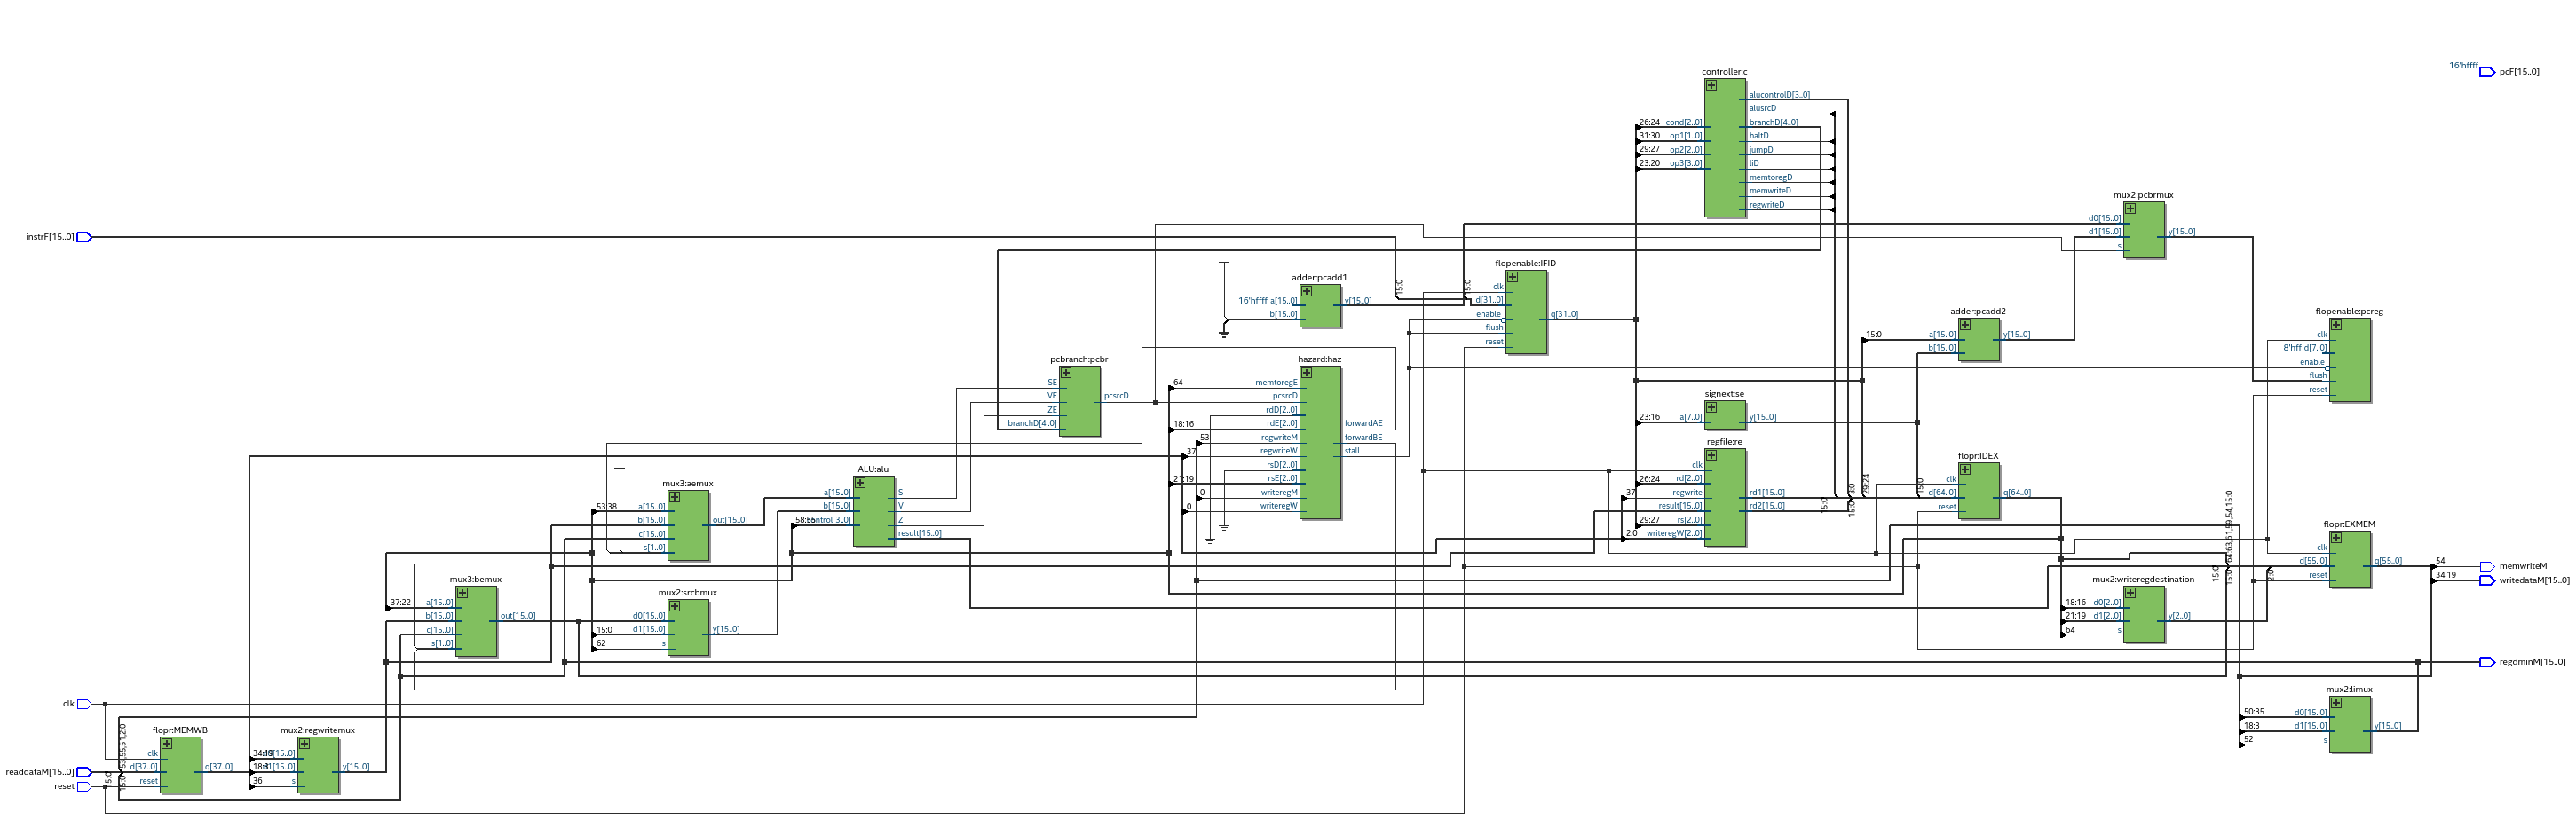
\includegraphics[width=15cm]{entire.png}
  \caption{QuartusRTLviewerのブロック図}
  \label{quartus}
\end{figure}
\begin{figure}[h]
  \centering
  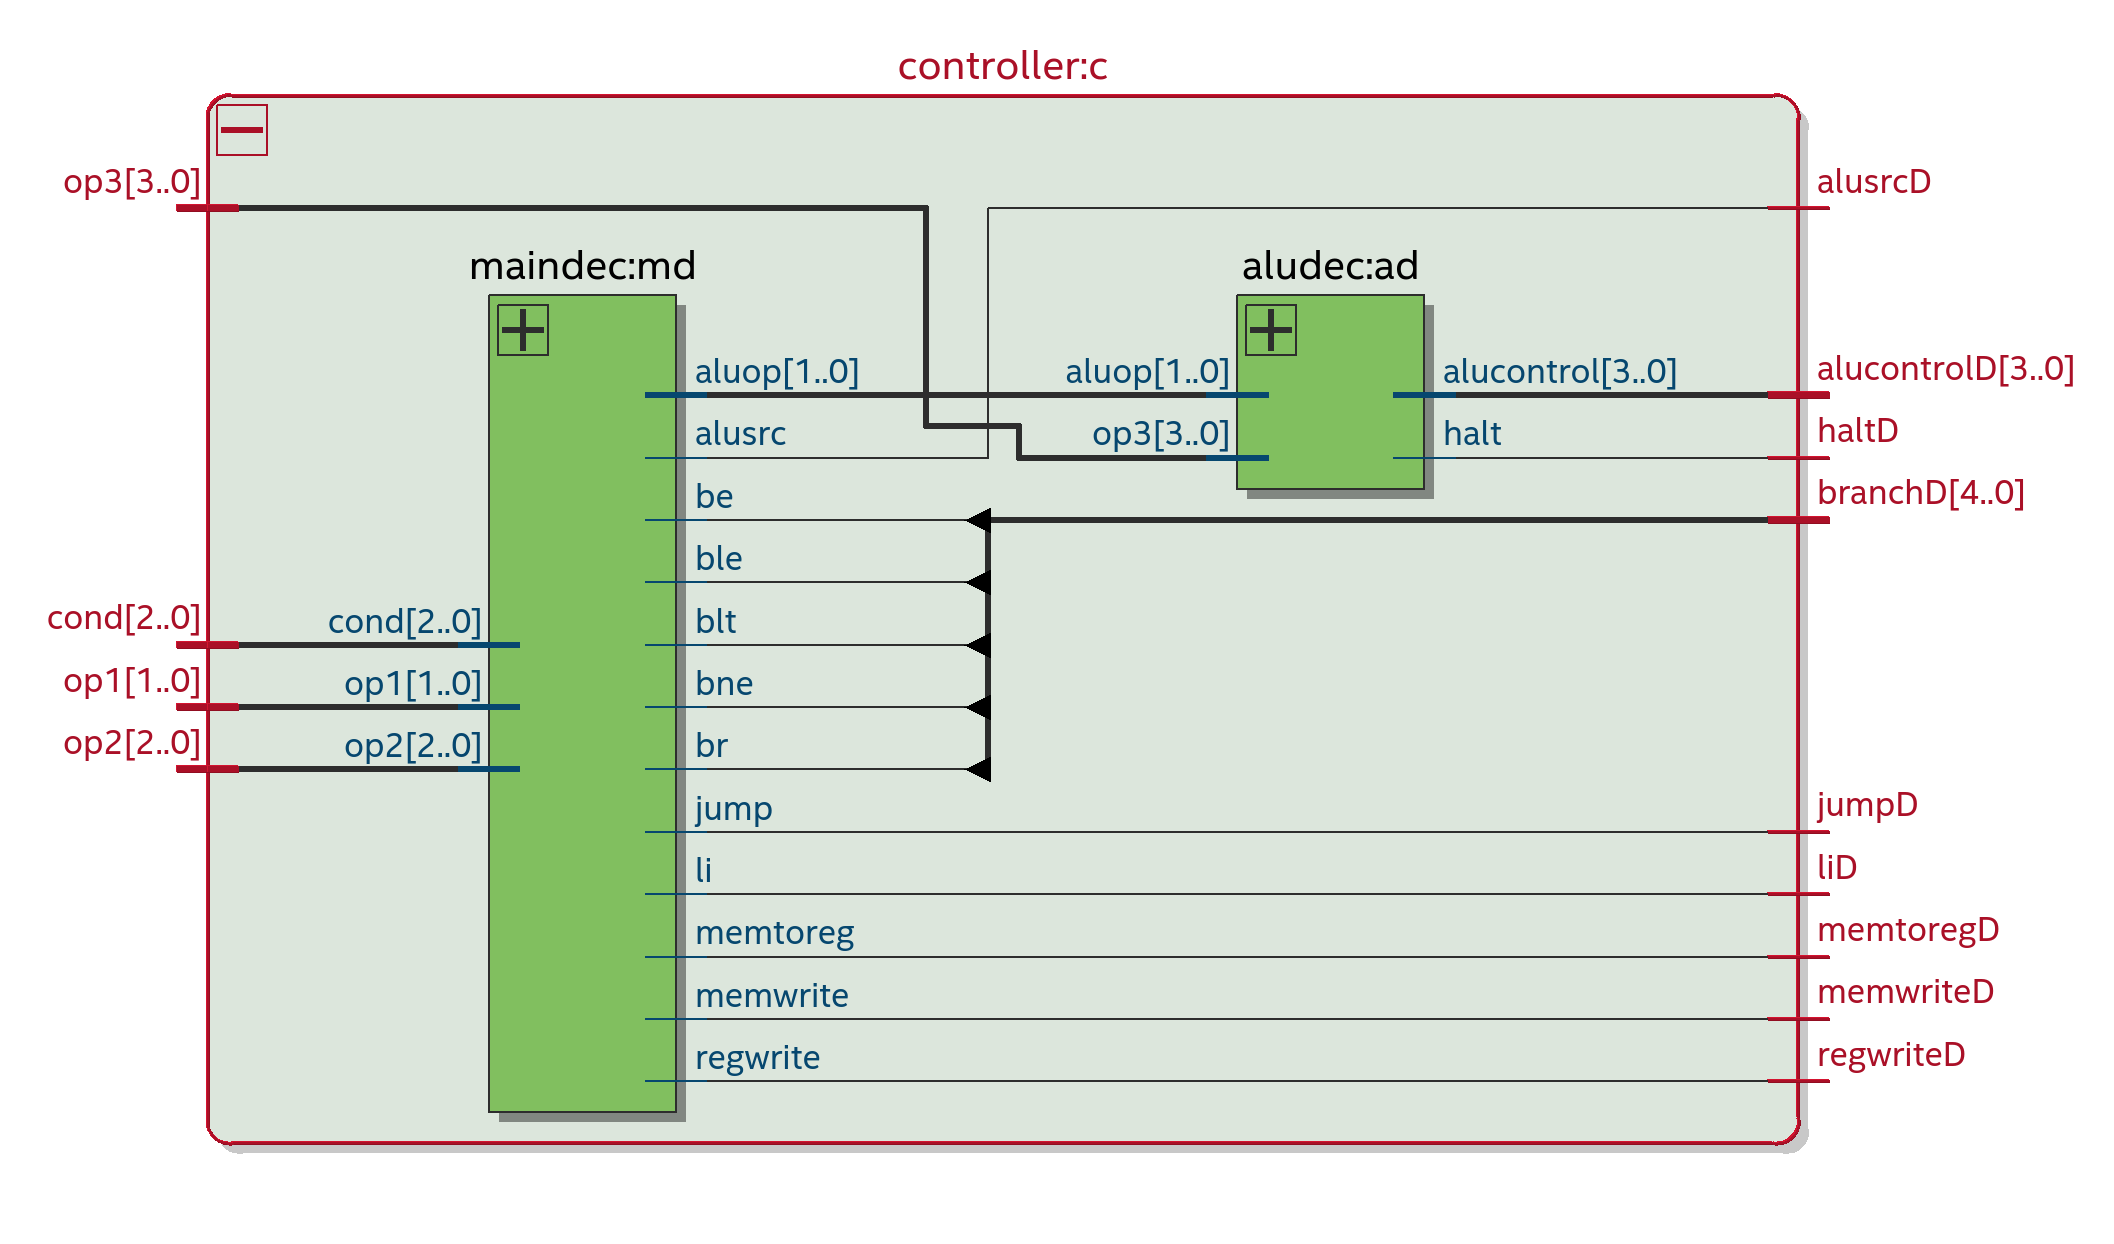
\includegraphics[width=10cm]{controller.png}
  \caption{制御部のブロック図}
  \label{contr}
\end{figure}
まず図\ref{block}のように全体をデータメモリモジュールDM、命令メモリモジュールIM、制御モジュールcontroller、ALUモジュールALU、マルチプレクサモジュールmux2、レジスタモジュールregfile、加算モジュールadder、プログラムカウンタ$\cdot$パイプラインレジスタモジュールflopr、符号拡張モジュールsignext、ブランチ制御モジュールbranch、ハザード検出ユニットhazard、フォワーディングユニットfowardingに分割している。更に制御モジュールcontrollerについては図\ref{contr}のようにメインデコーダーモジュールmaindecとALUデコーダーモジュールaludecの2つのモジュールから成り立っている。各レジスタ等はbit幅が違うものの図\ref{flopr}のように記述すること可変幅のインスタンスを作ることができ各パイプラインレジスタやマルチプレクサを別々のモジュールで作る必要がないように工夫した。分岐予測の実装については現段階では時間があれば行うことにしているので設計等はしていない。
\begin{figure}[h]
  \centering
  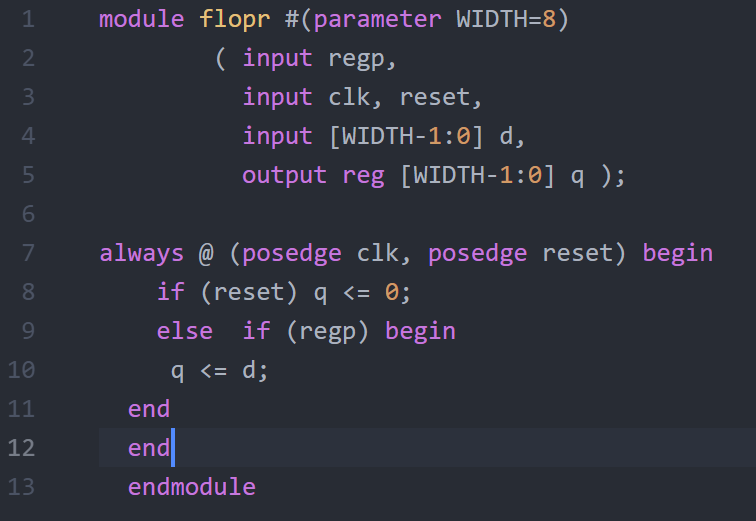
\includegraphics[width=10cm]{floprcode.png}
  \caption{可変長を指定できるインスタンス作成のコード例}
  \label{flopr}
\end{figure}

\newpage

\section{設計を担当するコンポーネントの外部仕様}
制御部以外の細かいモジュールの設計実装を担当したのでその周りの外部仕様を以下に示す。\\
\begin{itemize}
\item プログラムカウンタ前段のマルチプレクサはブランチ制御部から出力される信号pcsrcMが1のときブランチ命令で指定されたアドレスが出力されている信号pcbranchMを、pcsrcMが0のとき通常のPCに1足した値が出力されている信号pcplus1Eを信号pcに出力し、レジスタがフェッチしてくる次の命令のアドレスを指定する役割を持つ。
\item プログラムカウンタPCは上述のマルチプレクサで指定されたアドレスがpcから入力され次クロックでそれを信号pcnextに出力する。制御信号pcwriteが0のときはストールさせて値を読み出さない。
\item 命令メモリIMはプログラムカウンタから出力されたアドレスをpcnextから受け取りそのアドレスに書かれているバイナリの命令instrF[15:0]を出力する。この命令メモリにプログラムの命令列が入っていると考えて良い。
\item プログラムカウンタから出力されたアドレスpcnextは1加算され信号pcplus1Fに入力され前述のマルチプレクサとパイプラインレジスタIFIDに出力される。
\item パイプラインレジスタIFIDは命令メモリIMからの出力instrFと1加算されたアドレスpcplus1Fを受け取り次クロックでそれをそのままそれらをinstrDとpcplus1Dに出力する。プログラムカウンタと同様、IFIDwriteが0のときはストールさせて値を読み出さない。
\item レジスタregfileはinstrD[10:8]と instrD[13:11]を受け取りそのアドレスのレジスタに書き込まれている値をsrcaDとwritedataDに出力する。また制御部から入力される信号RegwiteDが1のとき入力writeregDが指定してるアドレスのレジスタにresultWから出力されている値を書き込む。
\item 符号拡張signextにはinstrD[7:0]が入力され符号拡張された値がsignimmDに出力される。
 \item 制御部controllerはinstrD[15:14]、instrD[13:11]、instrD[10:8]、instrD[7:4]を受け取りmemtoregD、memwriteD、branchD、alucontrolD、alusrcD、regwriteD、liDを出力する。memtoregDは命令がロードのとき1に、それ以外のときは0に設定される。memwriteDはストア命令のときに1に、それ以外のときは0に設定される。branchDは5bitの信号でそれぞれ命令がbe、blt、ble、bne、brのときに各桁が1に設定される。alucontrolDは4bitでその各値でALUで行う演算を指定する。alusrcDはロード命令とストア命令のときに1それ以外のときは0に設定される。regwriteDはALUで行う基本演算もしくは即値ロード含むロード命令のときに1に、それ以外のときには0に設定される。liDは即値ロードのとき1に、それ以外のときには0に設定される。これらの出力値はマルチプレクサに入力されストール時以外はこの入力がそのままマルチプレクサから出力される。
 \item パイプラインレジスタIDEXはsrcaD、writedataD、signimmD、pcplus1D、memtoregD、memwriteD、branchD、alucontrolD、alusrcD、regwriteD、liD、instrD[10:8]、instrD[13:11]を受け取り次クロックでこれらをそのままsrcaE、writedataE、signimmE、pcplus1E、memtoregE、memwriteE、branchE、alucontrolE、alusrcE、regwriteE、liE、instrE[10:8]、instrE[13:11]に出力する。
\item 次の命令メモリのアドレスを指すpcplus1Eは符号拡張されたsignimmEと加算されpcbranchEに出力される。
\item writedataEとsignimmEが入力されるマルチプレクサはその制御信号alusrcEが1のときsignimmEを、0のときwritedataEをwakaran1に出力する。
\item srcaE、resultW、regdminMが入力されるマルチプレクサは制御信号fowardAが00のときsrcaEを、01のときresultW、10のときregdminMをwakaran2に出力する。
\item wakaran1、resultW、regdminMが入力されるマルチプレクサは制御信号fowardBが00のときwakaran1を、01のときresultW、10のときregdminMをwakaran3に出力する。
 \item instrE[10:8]とinstrE[13:11]が入力されているマルチプレクサは制御信号memtoregEが1のときinstrE[13:11]を、0のときinstrE[10:8]をwriteregEに出力する。
\item ALUはwakaran2とwakara3を制御線alucontrolEの値に応じて各演算をしその結果をaluoutEに出力する。alucontrolEとその演算内容の対応については次頁図\ref{alu}に示す。またSIMPLE仕様書に定めれているとおりにSE、ZE、CE、VEを出力する。
\begin{figure}[h]
  \centering
  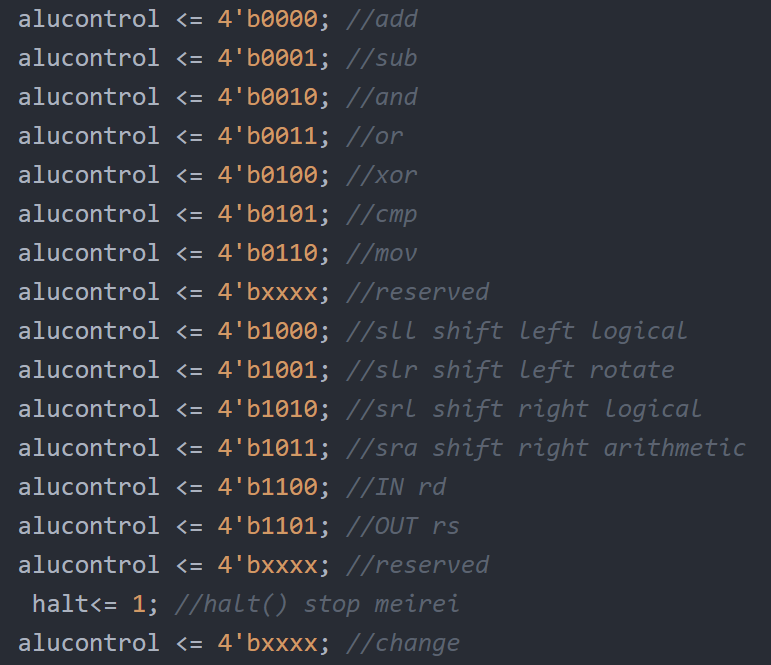
\includegraphics[width=10cm]{alucontrol.png}
  \caption{alucontrolEとその演算内容の対応}
  \label{alu}
\end{figure}

\item aluoutEとsignimmEが入力されるマルチプレクサはその制御信号liEが1のときsignimmEを、0のときaluoutEをregdminEに出力する。
\item パイプラインレジスタEXMEMはwritedataE、memtoregE、memwriteE、branchE、regwriteE、writeregE、pcbranchE、SE、ZE、CE、VE、regdminEを受け取り次クロックでこれらをそのままwritedataM、memtoregD、memwriteM、branchM、regwriteM、writeregM、pcbranchM、SM、ZM、CM、VM、regdminMに出力する。
\item データメモリDMはその制御線memwriteMが0のとき入力regdminMから入力されるアドレスの値をreaddataMに出力する。また制御線memwriteMが1のときはwritedataMに入力された値を入力regdminMから入力されるアドレスに保存する。
\item ブランチ制御モジュールbranchは制御信号branchM、SM、ZM、CM、VMを受け取り
pcsrcMを出力する。このpcsrcMは、branchMが示すどのブランチ命令を行うかと分岐を行う際の条件判定によりその出力値が0か1か決まる。例えばbranchMが今回の命令がBNEであることを示していてなおかつZが0の場合pcsrcMは1に設定される。
\item パイプラインレジスタMEMWBはmemtoregM、regwriteM、writeregM、readdataM、regdminMを受け取り次クロックでこれらをそのままmemtoregW、regwriteW、writeregW、readdataW、regdminWに出力する。
\item readdataWとregdminWが入力されているマルチプレクサはその制御信号memtoregWが1のときreaddataWを、0のときregdminWをresultWに出力する。
\end{itemize}

以上で自分が担当するコンポーネント周りの外部仕様の説明は終わる。フォワーディングユニット、ハザード検出、制御部、全てのコンポーネントを繋ぐ作業はペアの分担である。

\section{実装を担当するコンポーネントの内部仕様}
自分が担当したコンポーネントの内部仕様を記す。ただし我々の班は各コンポーネントをそれぞれひとつのモジュールに作ってそれらを別の一つのモジュールでまとめただけなので、深い階層構造になっておらず各コンポーネントはQuartus上で一つの論理回路で記述されるためブロック図を掲載することはできない。
\subsection{マルチプレクサ}
マルチプレクサはどの使用用途でも同じモジュールからインスタンス化出来るように汎用性の高い設計にした。具体的には入力のbit幅は可変で指定できるように工夫した。その記述方法は図\ref{flopr}の一行目と同様でparameterのあとの値を自由に設定できる。こうすることで様々な処理段階で使用できるマルチプレクサをひとつのモジュールで作ることが出来る。実装については三項演算子?:で一行で行える。
\subsection{加算器}
ALUで行わない加算をする際に用いる加算器。現在のプログラムカウンタに1足すときと、現在のプログラムカウンタ+1に分岐先の相対アドレスを足すときに用いる。こちらもverilogでは二項演算子+を用いて記述するだけなので特筆することはない。
\subsection{レジスタ}
クロックの立ち上がり時に書き込みを行い、クロックの逆位相を用いることで元のクロックの立ち下がりのときに読み出しを行う。こうすることでパイプライン化の際同じフェーズで読み出しと書き込みが同時に行える。書き込みについてはif文を用いてregwriteの制御線が1のときのみ書き込みを行うようにする。これもverilogの記述的には容易で前者はクロックclkの入力ごとに書き込みデータをレジスタにノンブロッキング代入し、
後者は逆位相のクロック\~clkの入力ごとに指定されたレジスタ内の内容を読み出す。
\subsection{符号拡張}
符号拡張への元の入力の最上位bitで符号拡張する部分を埋める。これもverilogの記述では入力a、符号拡張した出力yに対して\\
y = \{ \{8\{a[7]\}\}, a\} ;\\
のように簡単にかける。具体的にはa[7]がaの最上位bitを表しその値で上位8bitを埋める操作をしている。
\subsection{ALU}
制御線alucontrolEの値によって演算を行う。その対応表は図\ref{alu}の通り。
各演算についてどのような計算を行ったかは図\ref{op}に示す。この図での各行のオレンジ色の4bit値がalucontrolEの値に対応する。ADD、SUB、AND、OR XOR、CMP、MOV、については演算子とCの定義のままである。\par
 SLLはverilogの$<<$の演算子によりこの演算子の右のオペランドの値だけこの演算子の左側の値を符号なしで左シフトするのでこのように実現できる。
SLRについてはまず16-b[3:0]がbを16で割ったあまりであることから説明する。まず2進数bの各bitを下位bitから順に$a_0,\,a_1,\cdot\cdot\cdot ,\,a_{15}$とするとbの10進表現は
\begin{equation*}
\begin{split}
b_{10} &= 2^{15} \times a_{15} + 2^{14} \times a_{14} + \cdot\cdot\cdot + 2 \times a_1 + 1 \times a_0\\
&=16\times ( 2^{11}\times a_{15} + 2^{10} \times a_{14} + \cdot\cdot\cdot + 2 \times a_5 + 1 \times a_4) + 2^3 \times a_3 + 2^2 \times a_2 + 2 \times a_1 + 1 \times a_0\\
\end{split}
\end{equation*}
と表せる。したがって\\
$b_{10}\,mod(16) \equiv  2^3 \times a_3 + 2^2 \times a_2 + 2 \times a_1 + 1 \times a_0$\\
つまりb[3:0]はbの16で割ったあまりを示している。例えば$b_{10}=18のときこれを16で割ったあまりは2であり実際b[3:0]=0010となっている。よって(16-b[3:0])_{10}は14を表しこれに対して\{ a, a \} >> (16-b[3:0])という演算を行うとa$を2つつなげた32bitの値\{a,a\}を14だけ右にずらすということなので結果的にこれは左に2シフトしてあまりを右に補う操作と同値になる。以上がSLRの説明である。
SRLはSLLと同様でシフトの向きが逆なだけである。SRAはverilogの$>>>$が符号有りでシフトする演算なのでこのように記述できる。
\begin{figure}[h]
  \centering
  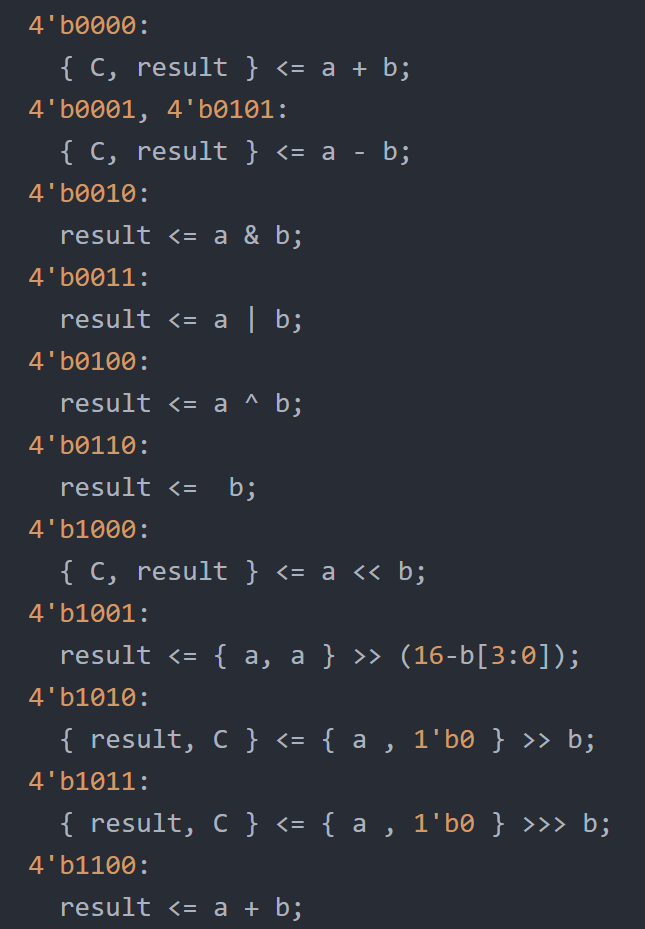
\includegraphics[width=7cm]{aluop.png}
  \caption{alucontrolEに対応する演算内容}
  \label{op}
\end{figure}
\subsection{パイプラインレジスタ}
これもマルチプレクサと同様、可変のparameterを用意する。特にパイプラインレジスタは改良の際にそのレジスタへの入力値の変更が起きやすいのでこのように設計することで改良がしやすかった。コンポーネントの役割は簡単でストール$\cdot$フラッシュの制御線が0のときはクロックごとに入力を出力にあたえるだけである。ストールの制御線が1のときは入力を出力に渡さないようにする。フラッシュの制御線が1のときは何も行わない信号を出力する。SIMPLEであれば1100\_0000\_0111\_0000などがreservedで何もしない命令となっている。
\subsection{メモリ}
データメモリDM、命令メモリIMともに枚クロックごとに読み込んだアドレスに格納されている値を出力する。データメモリについてはmemwriteMの値が1のときのみ入力writedataの値を入力アドレスに書き込む。
\subsection{ブランチ制御ユニット}
このユニットはALUで出力されたS、Z、C、Vと制御部からのbranch信号でpcsrsMを定める。branch信号はまず制御部からbranchD = \{be,blt,ble,bne,br\}としてverilogで記述され出力される。例えばbranchD = 00010の場合、今回の命令はBNEであることを示し、branchD = 00000なら今回の命令はbranch命令でないことを示す。これとS、Z、C、Vを用いることで例えばbranchD[0] \& ZE=1のときこれはBEの条件が成り立ちpcsrcMに1が出力される。このように (branchDの各bit)\&(そのbitが示す分岐が成立する条件コード)を羅列することでこれがpcsrcMが1になる条件となる。もちろんそれ以外のときはpcsrcMには0が設定される。


\end{document}
%todo: 全体画像とコントローラ画像の再読込、レジスタから出る信号線の確認l64,6971付近、ブランチ制御モジュールの名前は?branchのやつ逆では??
